% Chapter 5: Paisaje Competitivo
\chapter{Paisaje Competitivo}

\section{Análisis de Estructura de Mercado}
El mercado de consultoría de ingeniería minera se caracteriza por ser fragmentado y competitivo. Coexisten grandes firmas globales multidisciplinarias de ingeniería (con capacidades completas de EPCM) y firmas especializadas/boutique enfocadas en asesoría técnica de alto valor.

\begin{figure}[htbp]
\centering
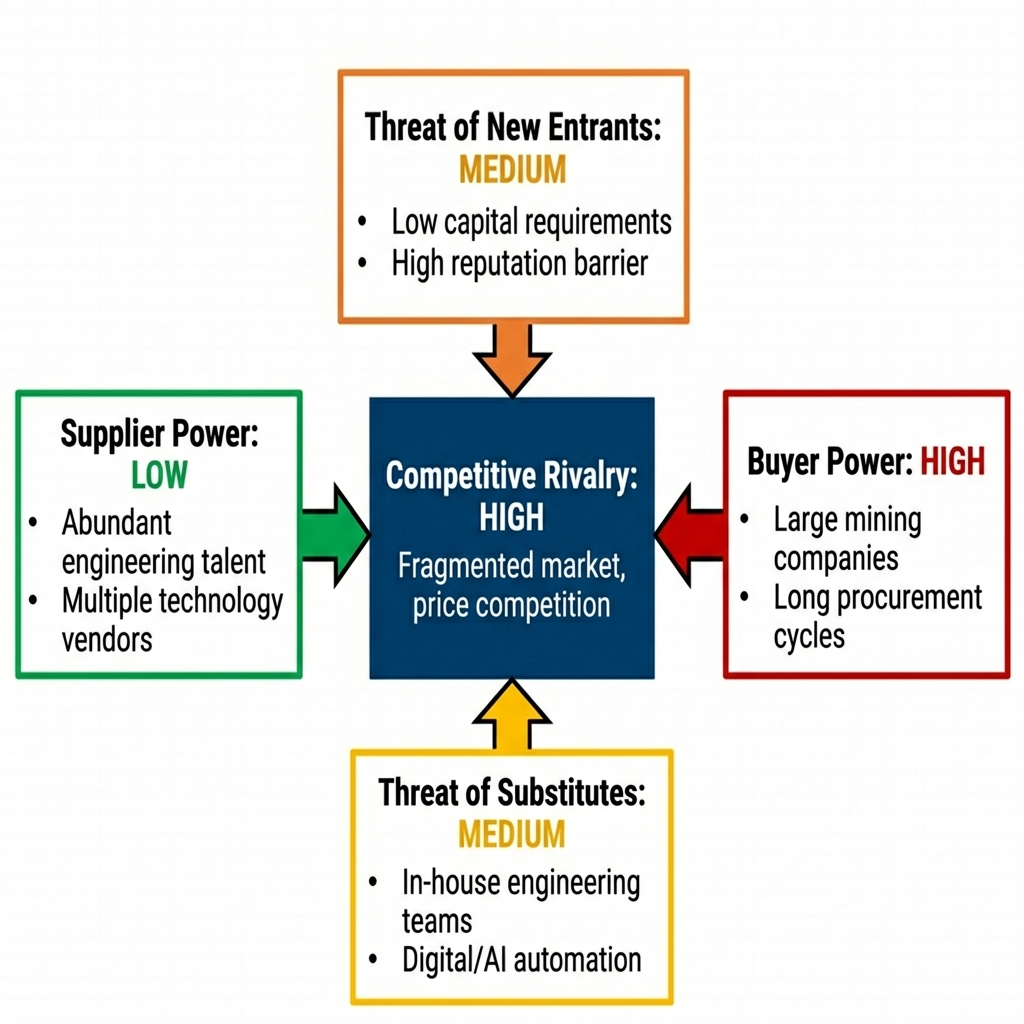
\includegraphics[width=0.88\textwidth]{../figures/03_porters_five_forces.png}
\caption{Análisis de las Cinco Fuerzas de Porter para el sector de Consultoría Minera.}
\label{fig:porter_forces}
\end{figure}

\begin{porterbox}[Resumen de las Cinco Fuerzas de Porter]
\begin{tabular}{@{}ll@{}}
\textbf{Fuerza} & \textbf{Clasificación} \\
\midrule
Rivalidad Competitiva & \riskhigh{} \\
Poder de Negociación de Proveedores & \risklow{} \\
Poder de Negociación de Clientes (Operadores) & \riskhigh{} \\
Amenaza de Nuevos Entrantes & \riskmedium{} \\
Amenaza de Sustitutos & \riskmedium{} \\
\end{tabular}
\end{porterbox}

\section{Mapeo y Comparación de Competidores Clave}

A continuación se perfilan los 5 competidores principales que definen las fronteras del mercado:

\begin{enumerate}
    \item \textbf{Worley (Público, ASX: WOR):}
    \begin{itemize}
        \item \textbf{Modelo de Negocio:} Gigante global de EPCM con ingresos agregados de AUD 12.05B en FY2025. Enfocado en grandes proyectos de infraestructura y energía.
        \item \textbf{Fortalezas:} Alcance global masivo, escala y capacidad de financiar proyectos gigantes de ejecución.
        \item \textbf{Debilidades:} Altos costos estructurales, menor agilidad para proyectos pequeños/medianos, burocracia.
        \item \textbf{Posicionamiento:} Líder global multidisciplinario.
    \end{itemize}

    \item \textbf{Hatch Ltd (Privado):}
    \begin{itemize}
        \item \textbf{Modelo de Negocio:} Corporación privada propiedad de sus empleados. Combina ingeniería pesada, gestión de proyectos y consultoría de procesos.
        \item \textbf{Fortalezas:} Profunda experiencia en metalurgia y procesos de procesamiento complejos; fuerte reputación de calidad.
        \item \textbf{Debilidades:} Menor escala que Worley, tarifas premium que limitan su competitividad en licitaciones de bajo costo.
        \item \textbf{Posicionamiento:} Consultoría técnica de alta complejidad e innovación.
    \end{itemize}

    \item \textbf{Jacobs Engineering Group (Público):}
    \begin{itemize}
        \item \textbf{Modelo de Negocio:} Proveedor de servicios profesionales completos, EPCM e inteligencia digital. Competidor cercano de Worley en el segmento corporativo.
        \item \textbf{Fortalezas:} Sólida presencia en EE.UU., fuerte enfoque en sostenibilidad y digitalización.
        \item \textbf{Debilidades:} Menos especializado en el nicho minero puro comparado con SRK o Hatch.
        \item \textbf{Posicionamiento:} Soluciones integrales de infraestructura y transición sostenible.
    \end{itemize}

    \item \textbf{SRK Consulting (Privado):}
    \begin{itemize}
        \item \textbf{Modelo de Negocio:} Grupo consultor internacional independiente y propiedad de sus empleados. Modelo basado estrictamente en asesoría técnica y diseño conceptual.
        \item \textbf{Fortalezas:} Máxima reputación científica/técnica en geología, geotecnia y planificación minera; neutralidad (no hacen construcción).
        \item \textbf{Debilidades:} No ofrecen servicios de construcción o EPCM a gran escala; dependen de consultores estrella.
        \item \textbf{Posicionamiento:} Especialista técnico independiente de referencia.
    \end{itemize}

    \item \textbf{Ausenco (Privado, PE-Backed):}
    \begin{itemize}
        \item \textbf{Modelo de Negocio:} Firma de ingeniería y EPCM respaldada por capital privado (Brightstar Capital). Especializada en soluciones eficientes y de rápido despliegue (ingeniería de bajo costo de capital).
        \item \textbf{Fortalezas:} Diseños de plantas altamente eficientes y modulares; agilidad y foco en la optimización de CAPEX para el cliente.
        \item \textbf{Debilidades:} Menor cobertura geográfica histórica; balance menos diversificado.
        \item \textbf{Posicionamiento:} Ingeniería ágil enfocada en maximizar el retorno de capital.
    \end{itemize}
\end{enumerate}

\section{Matriz de Posicionamiento Competitivo}

\begin{figure}[htbp]
\centering
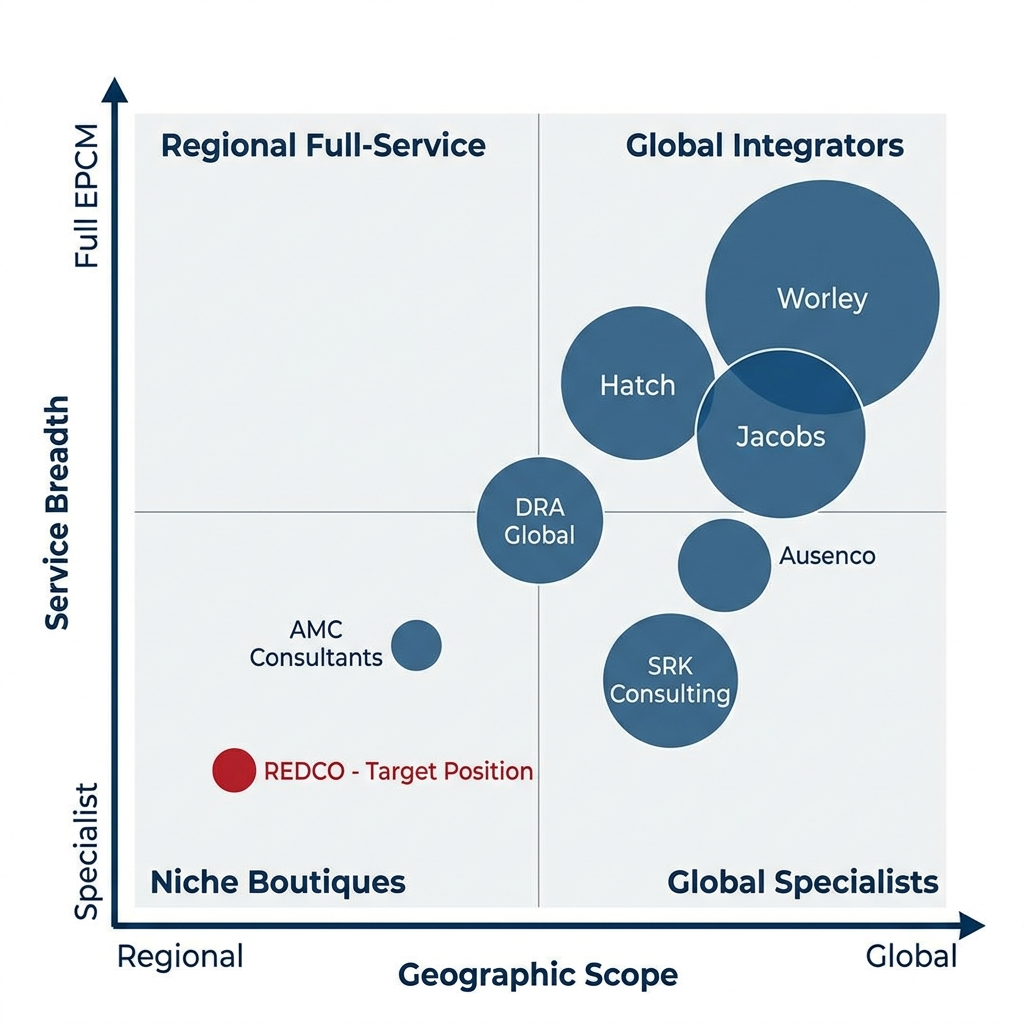
\includegraphics[width=0.88\textwidth]{../figures/04_competitive_positioning.png}
\caption{Matriz de Posicionamiento Competitivo 2x2. Eje X: Alcance Geográfico, Eje Y: Amplitud de Servicio.}
\label{fig:comp_matrix}
\end{figure}

El posicionamiento estratégico óptimo para REDCO se ubica en el cuadrante de \textbf{Niche Boutiques} (Boutiques de Nicho), con el objetivo de transicionar gradualmente hacia un rol de \textbf{Global Specialists} (Especialistas Globales) de nicho, apalancando la agilidad y la capacidad de responder a desafíos técnicos de alta especialidad que las grandes firmas de EPCM desatienden o sobrevaloran en precio.
